\documentclass[12pt,parskip]{komatufte}
\usepackage[subpreambles=false]{standalone}

%%%%%%%%%%%%%%%%%%%%%%%%%%%
% Silence warning messages
\usepackage{silence}
\WarningsOff[scrlayer-notecolumn]
\WarningsOff[biblatex]

%%%%%%%%%%%%%%%%%%%%
% Commenting

%\usepackage[author=Lyndon]{pdfcomment}
%\newcommand{\pdfcomment}[1]{} %ignore all comments

%\usepackage{todonotes}
%\newcommand{\pdfcomment}{\todo}


%%%%%%%%%%%%%%%%%%%%
% Tables
\usepackage{booktabs}

%%%%%%%%%%%%%%%%%%%
% Fonts
\usepackage{tgadventor} %sans
\usepackage{tgpagella}  %serif
\usepackage{inconsolata} %mono
\usepackage[T1]{fontenc}

\usepackage{microtype}
\usepackage[all]{nowidow}
%%%%%%%%%%%%%%%%%%%%%%%
% Styling
\setcounter{secnumdepth}{4}
\setcounter{tocdepth}{2}

\usepackage{placeins}



%%%%%%%%%%%%%%%%%%%
% Math
\usepackage{amsmath, amssymb, stmaryrd, mathtools}
\DeclareMathOperator*{\argmin}{argmin}
\DeclareMathOperator*{\argmax}{argmax}

\usepackage{xparse,xstring,etoolbox}
% crossref this against notation section
\newcommand{\vv}[1]{\tilde{#1}} % vector
\newcommand{\seq}[1]{\mathcal{#1}} % sequence
\newcommand{\set}[1]{\mathbb{#1}} % set

%%%%%%%%%
% Indexing/sequence indexing
\newcommand{\seqind}[2]{#1^{#2}} % seqence index
\newcommand{\ind}[2]{#1_{#2}} % indexed
\newcommand{\disamb}[2]{#1^{\mathrm{#2}}} %disambiguated

%% Smart indexing and naming
\newcommand{\ifupper}[3]{
    \normalexpandarg
	\exploregroups
	\StrCount{ABCDEFGHIJKLMNOPQRSTUVWXYZ}{#1}[\uppercount]
	\ifnumgreater{\uppercount}{0}{#2}{#3}
}

%smart index
\DeclareDocumentCommand{\ii}{u{_} m}{
	\ifupper{#1}%
	{% just a single uppercase character, i.e. a matrix
		  %make sure the index is the right length
		\StrCount{#2}{,}[\indcount]
		\ifnumgreater{\indcount}{0}
		{ % Got multiple indexes so all good
		 	\ind{#1}{#2}
		}
		{ % Only 1 index so grab the column
		 	\ind{#1}{{:,#2}}
		}
	}%
	{% Not just a single upper case character
		\ind{#1}{#2}
	}
}

\DeclareDocumentCommand{\nn}{u{_} m}{
	\seqind{#1}{#2}
}

\DeclareDocumentCommand{\dd}{u{_} m}{
	\disamb{#1}{#2}
}

% Index of a vector
\DeclareDocumentCommand{\iv}{u{_} m}{\ii{\vv #1}_{#2}}
\DeclareDocumentCommand{\dv}{u{_} m}{\dd{\vv #1}_{#2}}
\DeclareDocumentCommand{\nv}{u{_} m}{\nn{\vv #1}_{#2}}

%exp
\let\oldexp\exp
\renewcommand{\exp}[1]{\oldexp \left( #1 \right)}
\newcommand{\exptwo}[1]{\oldexp_2 \left( #1 \right)}

\newcommand{\softmax}{\mathrm{smax}}

\DeclareMathOperator*{\expectedop}{\mathbb{E}}
\DeclareDocumentCommand{\expected}{u{_} m}{
	\expectedop\limits_{\mathrlap{#2}}
}

%%%%%%%%%%%%%%%%
%Graphics
\usepackage{tikz}
\usetikzlibrary{positioning, fit,  shapes.geometric}
\usepackage{ifthen}
\usepackage{etoolbox}

\tikzset{
	backgroundcolor/.style ={fill=white},
	every node/.append style={
		minimum height=7mm,
	},
	labe/.append style={
		%Blue,
		align = center,
		backgroundcolor,
		fill opacity=0.6,
		text opacity=1,
		font={\footnotesize\itshape}	
	},
	layer/.append style={
		draw,
		align = center,
		minimum height=7mm,
	},
	tight/.append style={
		inner sep=0.2mm,
	},
	lookupbox/.append style={
		draw=none,
		append after command={
		       	[shorten <= -0.5\pgflinewidth]
		       	([shift={(-1.5\pgflinewidth,-0.5\pgflinewidth)}]\tikzlastnode.north east)
		       	edge([shift={( 0.5\pgflinewidth,-0.5\pgflinewidth)}]\tikzlastnode.north west) 
		       	([shift={( 0.5\pgflinewidth,-0.5\pgflinewidth)}]\tikzlastnode.north west)
		       	edge([shift={( 0.5\pgflinewidth,-1.5\pgflinewidth)}]\tikzlastnode.south west)            
		       	([shift={( -1.5\pgflinewidth,+0.5\pgflinewidth)}]\tikzlastnode.south east)
		       	edge([shift={(-1.5\pgflinewidth,-0.5\pgflinewidth)}]\tikzlastnode.north east)
		},
		inner sep=0.7mm,
		outer sep=0mm,
		minimum width=25mm
	}
}

\usepackage{pgfplots}
\pgfplotsset{compat=1.14}
\pgfplotsset{sideplot/.append style={
		width=\notescolwidth,
		domain=-10:10,
		samples=101,
		smooth,
		enlarge y limits={abs=2},
		axis lines=middle,
		xlabel  = $z$,
		ylabel  = $y$,
	},
	equ/.append style={
		color=blue,
		thick,
		mark=none
	}
}

% Function  For a plot 
% it  needs to be declared in preamble because of how \makenote* interacts with multiple files
\def\errorsurface(#1,#2){(0.5*#1 + 0.7*#2 + sin(deg(1.5*#1 + #2^2)))^2}


\usepackage{graphicx}
\graphicspath{{./figs/}, {./}, {./figs/chaptersentencerrepr/}, {./figs/chapterintromachinelearning/}, {./figs/chapterwordrepr/}}
\usepackage{adjustbox}


%%%%%%%%%%%%%%%%%%%
% Refs
\usepackage{cleveref}

\addbibresource{master.bib}

%%%%%%%%%%%%%%%%%%%%
% Formatting

% for examples from natural language space.
\newcommand{\natlang}[1]{\ifmmode \text{``\texttt{#1}''} \else {``\texttt{#1}''}\fi}
% \ifmmode ``trick'' from https://tex.stackexchange.com/a/15194/5834

%%%%%%%%%%%%%%%%%%%%%



\begin{document}

\setchapterpreamble{%
	\dictum[\textit{English Composition and Literature}, Webster, 1923]
	{
		A sentence is a group of words expressing a complete thought.
	}
}
\chapter{Sentence Representations and Beyond}\label{sec:sentence-representations-and-beyond}
\begin{abstract}
	Chapter 8: Sentence representations and beyond (5-10 pages)
	This chapter takes the previous discussion of phrases to the next level: sentences.
	This will include discussions of works on recursive structure
	As well work leveraging recurrent neural networks.
	Methods that do not strongly consider order (including Sum of Word Embeddings; paragraph vectors) will also be discussed here.
	Many of these techniques extent to arbitrary length sequences of words.
\end{abstract}


It can be argued that the core of true AI,
is the capture a machine manipulatable representation of an idea.
In natural language a sentence (as defined by Webster in the quote above),
is such a representation of an idea, but it is not machine manipulatable.
As such the conversion of sentences to a machine manipulatable representation is an important task in AI research.


All techniques which can represent documents (or paragraphs) can by necessity represent sentences as well.
A single sentence can be a whole document, similarly for paragraphs.
The reverse is not necessarily true: most documents are not just a single sentence.
When considering on documents beyond sentences,
neural network embedding models directly compete with vector information retrieval models.
These information retrieval models include LSI \pcite{dumais1988using}, probabilistic LSI \pcite{hofmann2000learning},  LDA \pcite{blei2003latent}.

\pdfcomment{I need to get my head straight about when these models are like word embeddings vs when they are like document embeddings. I think it is just taking on output instread of the other, but it has been a while since I looked at this}



\aside[Word Sense Embeddings as a by-product]{
Almost all sentence representation methods product word embeddings as a by-product
Either output embeddings, from softmax,
or input embeddings that are used as the networks inputs.}
\aside[Initialising input embeddings]{
In the case of systems with input embeddings it is common (but not ubiquitous) to initialised them using a pretrained embeddings from one of the methods discussed in the \Cref{sec:word-representations},
then allow them to be fine-tuned while training the sentence embeddings.
}

\section{Unordered and Weakly Ordered Representations}

\subsection{Sums of Word Embeddings}
\aside[SOWE is a BOW product]{
	The reader may recall from \Cref{sec:word-representations},
	that a word-embedding lookup is the same as a one-hot vector product:
	$C_{w_i} = C\,\hat{e}_{w_i}$.
	Similar can be said for sum of word embeddings (SOWE) and bag of words (BOW).
	For some set of words $\mathcal{W} = \lbrace{w_1,\ldots, w_n}$:
	the BOW representation is $B_\mathcal{W} = \sum_{w_i\in \mathcal{W}} \hat{e}_{w_i}$;
	the SOWE representation is $\sum_{w_i\in \mathcal{W}} C_{w_i} = CB_\mathcal{W}$.
	As with word-embeddings it is immensely cheaper to calculate this via lookup, than via matrix product;
	except on systems with suitable sparse matrix product tricks.	
}

Classically in information retrieval documents have been represented by bags of words (BOW).
That is to say a vector with length equal to the size of the vocabulary, with each position representing the count of the number of occurrences of a single word.
This is much the same as a one-hot vector representing a word, but with every word in the sentence/document counted.
The word embedding equivalent is sums of word embeddings (SOWE), and means of word embeddings (MOWE).
These methods, like BOW, lose all order information in the representation.
In many cases it is possible to recover a BOW from a much lower dimensional SOWE 

Surprisingly, they have been found on many tasks to be extremely well performing, better than several of the more advanced techniques discussed later in this chapter  \pcite{White2015SentVecMeaning}, \pcite{RitterPosition}.
It has been suggested that this is because in English there are only a few likely ways to order any given bag of words and thus original sentences can often be recovered from BOW \pcite{Horvat2014} and thus SOWE, \pcite{White2016a}, given a simple ngram language model.
The step beyond this is to encode the ngrams into a bag of words like structure.
The bag of ngrams (BON), e.g. bag of trigrams, has been classically used as an alternative to BOW.
Each index in the vector thus represents the occurrence of a ngram in the text.
So \natlang{It is a good day today}, has the 3grams: \natlang{(It is a)},\natlang{(is a good)},\natlang{(a good day)}, \natlang{(good day today)}.
As is obvious for all but the most pathological sentences, recovering the full sentence order from a bag of ngrams is possible even without a language model.

The natural analogy to this with word embeddings might seem to be to find ngram embeddings by the concatenation of $n$ word embeddings; and then to sum these.
However, such a sum is less informative than it might seem.
As the sum in each concatenated section is equal to the others, minus the edge words. To illustrate the case of trigram sums of word embeddings, for \natlang{It is a good day today},
the sums in each position would be:
\begin{align}
\left[\begin{array}{c|c|c}
	\sum & \sum & \sum\\
	C_{it} & C_{was} & C_{a}\\
	C_{was} & C_{a} & C_{good}\\
	C_{a} & C_{good} & C_{day}\\
	C_{good} & C_{day} & C_{today}
\end{array}\right]=\left[\begin{array}{c|c|c}
	C_{M}+C_{it}-C_{day} & C_{M} & C_{M}-C_{was}+C_{today}\end{array}\right]
\end{align}

\begin{align}
\left[\begin{array}{c|c|c}
	\quad C_{w_{1}} & \quad C_{w_{2}} & \quad C_{w_{3}}\\
	+C_{w_{2}} & +C_{w_{3}} & +C_{w_{4}}\\
	+C_{w_{3}} & +C_{w_{4}} & +C_{w_{5}}\\
	+C_{w_{4}} & +C_{w_{5}} & +C_{w_{6}}
\end{array}\right]=\left[\begin{array}{c|c|c}
	\sum C_{w_{i}}-C_{w_{n-1}}-C_{w_{n-2}} & \sum C_{w_{i}}-C_{w_{1}}-C_{w_{n-1}} & \sum C_{w_{i}}-C_{w_{1}}-C_{w_{2}}\end{array}\right]
\end{align}

\subsection{Paragraph Vector Models}

this work is an extension of \tcite{mikolov2012contextRNNLM}

\section{Sequential Models}

\subsection{Every RNN learns a sentence representation in its state}
\begin{figure}
	\caption{The unrolled structure of an RNN for us in Encoding, Decoding and Encoding-Decoding (sequence-to-sequence) problems. RU is the recurrent unit -- the neural network which reoccurs at each time step. (Repeated from \Cref{fig-rnns})
	}
	
	\label{fig-rnns-sq}
	
	\resizebox{\textwidth}{!}{\documentclass[landscape]{article}
\usepackage[a3paper]{geometry}

\usepackage{tikz}
\usetikzlibrary{positioning, fit,  shapes.geometric}
\usepackage{ifthen}
\usepackage{etoolbox}

\tikzset{
	backgroundcolor/.style ={fill=white},
	every node/.append style={
		minimum height=7mm,
	},
	labe/.append style={
		%Blue,
		align = center,
		backgroundcolor,
		fill opacity=0.6,
		text opacity=1,
		font={\footnotesize\itshape}	
	},
	layer/.append style={
		draw,
		align = center,
		minimum height=7mm,
	},
	tight/.append style={
		inner sep=0.2mm,
	},
	lookupbox/.append style={
		draw=none,
		append after command={
		       	[shorten <= -0.5\pgflinewidth]
		       	([shift={(-1.5\pgflinewidth,-0.5\pgflinewidth)}]\tikzlastnode.north east)
		       	edge([shift={( 0.5\pgflinewidth,-0.5\pgflinewidth)}]\tikzlastnode.north west) 
		       	([shift={( 0.5\pgflinewidth,-0.5\pgflinewidth)}]\tikzlastnode.north west)
		       	edge([shift={( 0.5\pgflinewidth,-1.5\pgflinewidth)}]\tikzlastnode.south west)            
		       	([shift={( -1.5\pgflinewidth,+0.5\pgflinewidth)}]\tikzlastnode.south east)
		       	edge([shift={(-1.5\pgflinewidth,-0.5\pgflinewidth)}]\tikzlastnode.north east)
		},
		inner sep=0.7mm,
		outer sep=0mm,
		minimum width=25mm
	}
}
\usepackage{amsmath, amssymb, stmaryrd, mathtools}
\DeclareMathOperator*{\argmin}{argmin}
\DeclareMathOperator*{\argmax}{argmax}

\usepackage{xparse,xstring,etoolbox}
% crossref this against notation section
\newcommand{\vv}[1]{\tilde{#1}} % vector
\newcommand{\seq}[1]{\mathcal{#1}} % sequence
\newcommand{\set}[1]{\mathbb{#1}} % set

%%%%%%%%%
% Indexing/sequence indexing
\newcommand{\seqind}[2]{#1^{#2}} % seqence index
\newcommand{\ind}[2]{#1_{#2}} % indexed
\newcommand{\disamb}[2]{#1^{\mathrm{#2}}} %disambiguated

%% Smart indexing and naming
\newcommand{\ifupper}[3]{
    \normalexpandarg
	\exploregroups
	\StrCount{ABCDEFGHIJKLMNOPQRSTUVWXYZ}{#1}[\uppercount]
	\ifnumgreater{\uppercount}{0}{#2}{#3}
}

%smart index
\DeclareDocumentCommand{\ii}{u{_} m}{
	\ifupper{#1}%
	{% just a single uppercase character, i.e. a matrix
		  %make sure the index is the right length
		\StrCount{#2}{,}[\indcount]
		\ifnumgreater{\indcount}{0}
		{ % Got multiple indexes so all good
		 	\ind{#1}{#2}
		}
		{ % Only 1 index so grab the column
		 	\ind{#1}{{:,#2}}
		}
	}%
	{% Not just a single upper case character
		\ind{#1}{#2}
	}
}

\DeclareDocumentCommand{\nn}{u{_} m}{
	\seqind{#1}{#2}
}

\DeclareDocumentCommand{\dd}{u{_} m}{
	\disamb{#1}{#2}
}

% Index of a vector
\DeclareDocumentCommand{\iv}{u{_} m}{\ii{\vv #1}_{#2}}
\DeclareDocumentCommand{\dv}{u{_} m}{\dd{\vv #1}_{#2}}
\DeclareDocumentCommand{\nv}{u{_} m}{\nn{\vv #1}_{#2}}

%exp
\let\oldexp\exp
\renewcommand{\exp}[1]{\oldexp \left( #1 \right)}
\newcommand{\exptwo}[1]{\oldexp_2 \left( #1 \right)}

\newcommand{\softmax}{\mathrm{smax}}

\DeclareMathOperator*{\expectedop}{\mathbb{E}}
\DeclareDocumentCommand{\expected}{u{_} m}{
	\expectedop\limits_{\mathrlap{#2}}
}

\begin{document}

\numdef{\N}{8}
\numdef{\labelwidth}{5.5cm}
%%%%%%%%%%%%%%%%%%%%%%%%%
% Encoder

\begin{tikzpicture}[]

\begin{scope}
	\node(lblEncoder)[text width= \labelwidth] {\textbf{RNN Encoder:}\\%
	Variable $n$ inputs: $\nv x_t$\\%
	1 output: $\hat{y}$ \\%
	};
	
	\coordinate (L0) at (lblEncoder.east);
	
	\foreach \I[count=\j from 0] in {1,...,\N}{
		\ifnumequal{\I}{\N - 1}{%
			\node(L\I)[dashed, layer, right = of L\j] {...};
			\node(w\I)[below = of L\I]{...};
		}%
		{	
			\node(L\I)[layer, right = of L\j] {RU};
			\node(w\I)[below = of L\I]{\ifnumequal{\I}{\N}{$\nv x_n$}{$\nv x_\I$}};
			\draw[->](w\I) -- (L\I);
		}
	}
	\foreach \I[count=\j from 1] in {2,...,\N} {
		\draw[->] (L\j) edge node[labe]{state} (L\I);
	}
	
	\node(out) [above = of L\N]{$\hat{y}$};
	\draw[->] (L\N) -- (out);
\end{scope}

%%%%%%%%%%%%%%%%
% Decoder
\begin{scope}[yshift=-5cm] 
\node(lbl)[text width= \labelwidth] {\textbf{RNN Decoder:}\\%
1 input: $x$\\%
variable $m$ outputs: $\n \hat{y}_t$ \\%
with prompts: $\nv r_t$ (often $\nv y_{t-1}$)
};

\coordinate (L0) at (lbl.east);
\coordinate (L1c)[right = of L0];
\node(x)[below right = 4 of L1c]{$x$};

\foreach \I[count=\j from 0] in {1,...,\N}{
	\ifnumequal{\I}{\N - 1}{%
		\node(L\I)[dashed, layer, right = of L\j] {...};
		\node(w\I)[above = of L\I]{...};
		\node(y\I)[below = of L\I]{...};
	}%
	{	
		\node(L\I)[layer, right = of L\j] {RU};
		\node(v\I)[above = of L\I]{\ifnumequal{\I}{\N}{$\n \hat{y}_m$}{$\n \hat{y}_\I$}};
		\node(w\I)[below = of L\I]{$[\nv r_\I; \v x]$};
		\draw[->](w\I) -- (L\I);
		\draw[->](L\I) -- (v\I);
		\draw[->](x) to[bend right = 5] (w\I.300);
	}
}
\foreach \I[count=\j from 1] in {2,...,\N} {
	\draw[->] (L\j) edge node[labe]{state} (L\I);
}

\end{scope}
%
%%%%%%%%%%%%%%%%%%
% Encoder Decoder
%
\begin{scope}[yshift=-14cm]
\node(lbl)[text width= \labelwidth] {\textbf{RNN Encoder-Decoder:}\\%
Variable $n$ inputs: $\nv x_t$\\%
Variable $m$ outputs $\n \hat{y}_t$\\%
Prompts: $\nv r_t$ (often $y_{t-1}$)
};

\coordinate (L0) at (lbl.east);
\numdef{\NN}{4}
\foreach \I[count=\j from 0] in {1,...,\NN}{
	\ifnumequal{\I}{\NN - 1}{%
		\node(L\I)[dashed, layer, right = of L\j] {...};
		\node(w\I)[below = of L\I]{...};
	}%
	{
		\node(L\I)[layer, right = of L\j] {$\mathrm{RU_E}$};
		\node(w\I)[below = of L\I]{\ifnumequal{\I}{\NN}{$\nv x_n$}{$\nv x_\I$}};
		\draw[->] (w\I) -- (L\I);
	}
}
\foreach \I[count=\j from 1] in {2,...,\NN} {
	\draw[->] (L\j) edge node[labe] {state} (L\I);
}




\coordinate[above = 3 of L\NN] (Lp\NN);
\numdef{\NP}{\N - 1}
\foreach \j in {\NN,...,\NP}{
	\numdef{\I}{\j+1}
	\numdef{\y}{\I - \NN}
	\ifnumequal{\I}{\N-1}{%
		\node(Lp\I)[dashed, layer, right = of Lp\j] {...};
		\node(w\I)[below = of Lp\I]{...};
		\node(y\I)[above = of Lp\I]{...};
	}%
	{
		\node(Lp\I)[layer, right = of Lp\j] {$\mathrm{RU_D}$};
		\ifnumequal{\I}{\N}{
			\node(w\I)[below = of Lp\I]{$[\v z; \nv r_m]$};
			\node(y\I)[above = of Lp\I]{$\n \hat{y}_m$};
		}
		{
			\node(w\I)[below = of Lp\I]{$[\v z; \nv r_\y]$};
			\node(y\I)[above = of Lp\I]{$\n \hat{y}_\y$};
		}

		\draw[->] (w\I) -- (Lp\I);
		\draw[->] (Lp\I) -- (y\I);
		\path[->] (L\NN.north) edge node[labe]{$\v z$} (w\I.south west);
	}
}


\numdef{\NNp1}{\NN + 1}
\foreach \I in {\NNp1,...,\NP} {
	\numdef{\j}{\I+1}
	\draw[->] (Lp\I) edge node[labe] {state} (Lp\j);
}
 

\end{scope}


\end{tikzpicture}




\end{document}}
\end{figure}

The majority of this section draw on the recurrent neural networks (RNN) as discussed in \Cref{sec:rnn}.
We can used RNN encoders and decoders (as shown in \Cref{fig-rnns-sq}) to generate representations of sequences by extracting a coding layer.
In one can take any RNN encoder,
and select the one of the hidden layers after the final recurrent unit (RU) that has processed the last word in the sentence.
Similarly for any RNN decoder, one can select any hidden layer before the first recurrent unit that begins to produce words.
For an RNN encoder-decoder, this means selecting the hidden layer from between.
As for example in \tcite{cho-EtAl:2014:EMNLP2014}.

\subsection{VAE and encoder-decoder}
\tcite{Bowman2015SmoothGeneration} presents an extension on this notion,
where in-between the encoder and the decode stages there is a variational autoencoder (VAE).
The variational autoencoder \pcite{2014VAE} an autoencoder that has been demonstrated to have very good properties in a number of machine learning applications.
Using the VAE it is hoped that a better representation can be found for the sequence of words in the input and output.

As shown in \Cref{fig:bowman}.

Bowman et. al. training there network as encoder-decoder for English.
The VAE is the hidden coding layer. 
They found that short syntactically similar sentences were located near to each other according to this space.
Further the that, because it has a decoder, it can generate these nearby sentences.

\begin{figure}
	\caption{The VAE plus encoder-decoder of \textcite{Bowman2015SmoothGeneration}.
		Note that during training, $\hat{y}_i=w_i$, as it is an autoencoder model,
		and as is normal for encoder-decoders the prompts are the previous output (target during training, predicted during testing) $r_i=y_{i-1}$,
		with $r_1=y_0=<EOS>$ being a pseudo-token marker for the end of string.
	}
	\label{fig:bowman}
	
	
	%%%%%%%%%%%%%%%%%%%%%%%%%
	% Encoder
	\resizebox{\textwidth}{!}{\begin{tikzpicture}[]
		\coordinate (L0) at (lbl.east);
		
		\node(L1)[layer, right = of L0] {$\mathrm{RU_E}$};
		\node(w1)[below = of L1]{$w_1$};
		\draw[->] (w1) -- (L1);
	
		\node(L2)[layer, right = of L1] {$\ldots$};
		\node(w2)[below = of L2]{$\ldots$};
	
		\node(L3)[layer, right = of L2] {$\mathrm{RU_E}$};
		\node(w3)[below = of L3]{$w_n$};
	
		\node(L4)[layer, above = of L3] {$VAE$};
		
		
		\node(L5)[layer, above right = of L4] {$\mathrm{RU_D}$};
		\node(w5)[below = of L5]{$r_1$};
		\node(y5)[above = of L5]{$\hat{y}_1$};
		\draw[->] (L5) -- (y5);
		
		\node(L6)[layer, right = of L5] {$\ldots$};
		\node(w6)[below = of L6]{$\ldots$};
		\node(y6)[above = of L6]{$\ldots$};
		\draw[->] (L6) -- (y6);
		
		
		\node(L7)[layer, right = of L6] {$\mathrm{RU_D}$};
		\node(w7)[below = of L7]{$r_m$};
		\node(y7)[above = of L7]{$\hat{y}_m$};
		\draw[->] (L7) -- (y7);
		\draw[->] (w7) -- (L7);
		
		
		\foreach \i/\j in {1/2, 2/3, 5/6,6/7} {
			\draw[->] (L\i) edge node[labe] {state} (L\j);
			\draw[->] (w\i) -- (L\i);
		}
		\draw[->] (L3) edge node[labe] {output} (L4);		
		\draw[->, bend left] (L4) edge node[labe] {output} (L5);
		 
	\end{tikzpicture}}
	
\end{figure}

\subsection{Skip-thought}
\tcite{DBLP:journals/corr/KirosZSZTUF15} draws inspiration from language modelling, to attempt to predict the previous and next sentence as an task.
They use an Encoder-Decoder RNN, with two decoder parts.
One decoder is to produce the previous sentence.
The other decoder is to produce the next sentence.

\begin{figure}
	\caption{The skip-thought model \textcite{DBLP:journals/corr/KirosZSZTUF15}.}
	\label{fig:skip-thought}
	
	%%%%%%%%%%%%%%%%%%%%%%%%%
	% Encoder
	\resizebox{\textwidth}{!}{\begin{tikzpicture}[]
		\coordinate (L0) at (lbl.east);
		
		\node(L1)[layer, right = of L0] {$\mathrm{RU_E}$};
		\node(w1)[below = of L1]{$w_1$};
		\draw[->] (w1) -- (L1);
		
		\node(L2)[layer, right = of L1] {$\ldots$};
		\node(w2)[below = of L2]{$\ldots$};
		
		\node(L3)[layer, right = of L2] {$\mathrm{RU_E}$};
		\node(w3)[below = of L3]{$w_n$};
		

		\node(LN5)[layer, above right = 2 of L3] {$\mathrm{RU_N}$};
		\node(LP5)[layer, below right = 2 of L3] {$\mathrm{RU_P}$};
		\foreach \d in {N,P} {
			\draw[->] (L3.east) edge node[labe] {state} (L\d5.west);
					
			\node(w\d5)[below = of L\d5]{$r_{\d, 1}$};
			\node(y\d5)[above = of L\d5]{$\hat{y}_{\d, 1}$};
			\draw[->] (L\d5) -- (y\d5);
			
			\node(L\d6)[layer, right = of L\d5] {$\ldots$};
			\node(w\d6)[below = of L\d6]{$\ldots$};
			\node(y\d6)[above = of L\d6]{$\ldots$};
			\draw[->] (L\d6) -- (y\d6);
			
			
			\node(L\d7)[layer, right = of L\d6] {$\mathrm{RU_\d}$};
			\node(w\d7)[below = of L\d7]{$r_{\d, m}$};
			\node(y\d7)[above = of L\d7]{$\hat{y}_{\d, m}$};
			\draw[->] (L\d7) -- (y\d7);
			\draw[->] (w\d7) -- (L\d7);	
		}


				
		\foreach \i/\j in {1/2, 2/3, N5/N6, N6/N7, P5/P6, P6/P7} {
			\draw[->] (L\i) edge node[labe] {state} (L\j);
			\draw[->] (w\i) -- (L\i);
		}
		

		
		\end{tikzpicture}}
	
\end{figure}


\section{Structured Models}
\aside[Parsers]{There are many high-quality parsing libraries available.
	Of particular note is the Stanford parser, included in Core NLP.
	It has bindings in many languages, including Python via NLTK.
	It has an interactive web-demo at \url{http://corenlp.run/},
	which was used to produce \Cref{fig:consparse,fig:depparse}
}

A limitation of sequential models is information only flows in a sequence.
However, the actual structure of natural language is not so simple.
Linguists tend to break sentences down into a tree or graph structure.
This is referred to as parsing.
The two most common are constituency parse trees, and dependency parse trees.
Examples of each are shown in \Cref{fig:consparse,fig:depparse}
It is beyond the scope of this book to explain the precise meaning of these trees.
The essence is that that represent the structure of the sentence,
according to how linguists currently understand how sentences are processed by humans.
The constituency parse breaks the sentence down into parts such as noun phrase (NP) and verb phrase (VP),
which are in turn broken down into phrases, or (POS tagged) words.
The constituency parse is well thought-of as a hierarchical breakdown of a sentence into its parts.
Conversely, a dependency parse is better thought of as a set of binary relations between head-terms and there dependent terms, though this likewise does result in a tree structure.
These structures are well linguistically motivated, so it make sense to use them in the processing of natural language.

\begin{figure}
	\caption{A constituency parse tree for the sentence \natlang{This is a simple example of a parse tree}}
	\centering{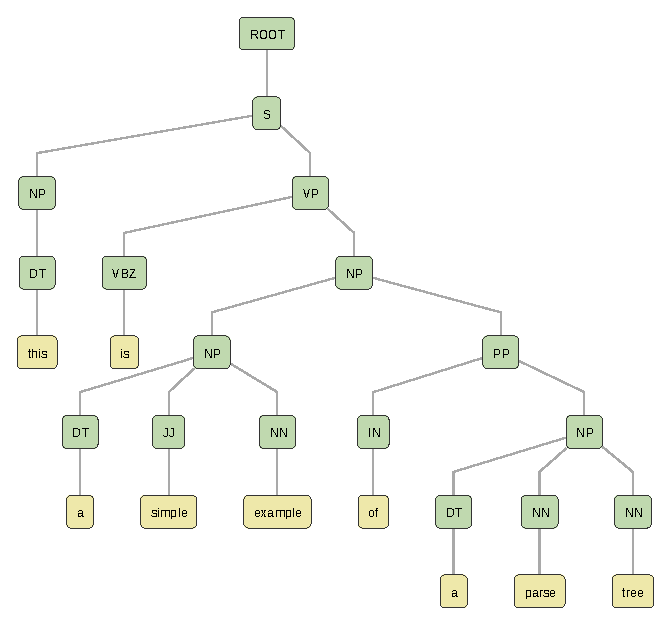
\includegraphics[width=\textwidth]{constparse}}
	\label{fig:consparse}
\end{figure}


\begin{figure}
	\caption{A dependency parse tree for the sentence \natlang{This is a simple example of a parse tree},
	This flattened view may be misleading.
	\natlang{example} is at the peak of the tree, with direct children	being:
	\natlang{this},\natlang{is},\natlang{a},\natlang{simple},
	and \natlang{tree}.
	\natlang{tree} has direct children being: \natlang{of},\natlang{a}, and \natlang{parse}.
}
	\centering{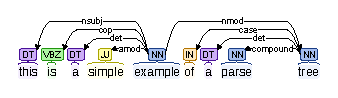
\includegraphics[width=\textwidth]{depparse}}
	\label{fig:depparse}
\end{figure}


\aside[Machine learning frameworks for structural models]{
	Structural networks can not be defined in most modern static neural network frameworks,
	such as TensorFlow.
	These frameworks function by defining a single computational graph that is used to process each training/test case.
	The same graph is used for each input.
	By definition the structure of the network differs from training/test case to training/test case.
	Technically the same problems apply to RNNs, as each case can have a different number of inputs.
	This is normally worked around by defining the network graph for the longest input to be considered,
	then padding all the inputs to this length.
	Such is not possible with structured networks.
	Other tricks are possible but are significantly more difficult.
	The exception to this is of-course via dynamic components to the static frameworks
	(which TensorFlow and other such frameworks certainly do have).
	Even in a dynamic tool it remains a non-trivial task to implement these networks.
}


\aside[Implementing Back-propagation through structure]{
	Back-propagation through structure is conceptually not significantly more complex than back propagation through time,
	in practice a very difficult algorithm to get right.
	In implementation it is very important to test for correctness using gradient checks, as it is easy to make a mistake and end-up with models that seem to work ok, but are actually crippled due to some mistake in the coding.
	Unfolding recursive autoencoders are particularly difficult,
	as the gradient must be propagated from all leaves.
	And output interior nodes can not have there gradients calculated until the gradients of their children are calculated.
	The solution to this is to process the gradients using a priority queue,
	where the priority is set by the depth of the node.
	Thus ensuring all children are processes before there parents.
}


We refer here to models incorporating tree, or graph structures as structural models.
Particular different variations have there own names, such as recursive neural networks (RvNN), and recursive autoencoders (RAE).
We use the term structural model as an all encompassing term. 
It also makes for clearer reading to distinguish recursive and recurrent  neural networks.
Just as a linked list is but a particular case of a tree, an RNN is a particular case of a structural model,
however we will exclude them from this discussion except where marked.


The initial recent work on structural models was done in for the thesis of \tcite{socher2014recursive}.
It builds on the work of \tcite{goller1996BPstructure} and \tcite{Pollack199077}, which presents back-propagation through structure.
Back-propagation can be applied to networks of any structure, much like (and indeed directly because) the chain-rule can be applied to any equation to find its derivative.
This means that structuring a network according to its parse structure is possible.


These tree structured networks function apply an recursive unit (which we will call RV) across pairs (or other groups of) the representations of the lower levels, to produce a combined representation.
For the example of a network which handles binary tree inputs the RV would be:

\begin{align}
	f_{RV}(u, v) &= \varphi\left( [S;R][u;v] + b \right) \\
			     &= \varphi\left( Su +Rv + b \right)
\end{align}

where $u$ and $v$ are the left and right substructures embeddings (word embeddings at the leaf node level), and $S$ and $R$ are the matrices defining the left and right inputs are to be combined.

This is a useful form as all constituency parse trees are commonly converted into binary parse trees, via left-factoring or right factoring (adding new nodes to the left or right to take some of the children).
This is sometimes call putting binarization, or putting them into  Chomsky normal form.
This form was used in \tcite{socher2010PhraseEmbedding}, \tcite{SocherEtAl2011:RAE},  \tcite{SocherEtAl2011:PoolRAE},
 \tcite{Socher2011ParsingPhrases} and \tcite{zhang2014BRAE}.
Where the $S$ and $R$ matrices are shared for all words.

This is in-contrast to \tcite{iyyer2014generating} and \tcite{socherDTRNN}, which works over dependency parse trees.
In this network nodes could have many inputs.
But depending on the relationship, eg \natlang{nsub}, \natlang{det}, \natlang{nmod}, \natlang{case}, a different matrix was used.
For $r(i,j)$ giving the relationship between word $i$ and the $j$, where $i$ is the head word, according to the dependency parse,
the following expressing gives the 

\begin{align}
	f_{RV}(i) &= \varphi\left(W_{head} C_{w_i} + \sum_{j \in \mathrm{children}(i)} W_{r(i,j)} \, f_{RV}(j) + b \right)
\end{align}

where $C_{w_i}$ is the word embedding for $w_i$.
Note that the terminal case is when a node has no children, which is just $f_{RV}(i) = \varphi \left( W_{head} C_{w_i} + b \right)$.




In \textcite{socherDTRNN}, an a similar network was used for projecting text captions into a common vector space where they would be near to there images.
The network was first trained to on an accusal language modelling task \pdfcomment{Need to get some more details on this bit}.
Then once it was trained its weights were locked and a separate CNN was trained to produce image representations such that those representations were near (in vector space) to the sentence's embeddings.


A similar technique of multiple inputs distinguished by using different matrices based on there relationship to the whole phrase,
 could be applied to non-binary constituency part trees.
This would be using the part of speech (e.g. VBZ, NN) and phrase tags (e.g. NP, VP) for the substructures to choice the weight matrix, to be applied to the embedding that is determined by the input from below (word embedding in the leaf nodes).
This would however lose order information in some cases.

The next step along this line of reasoning is to allow the input below to not only determine the embedding vector input but also to determine the matrices used to encode the relationship.
So not only is the representation of the (sub)prase determined by a relationship between  its constituents (as represented by there embeddings),
but the nature of that relationship (as represented by the matrix) is also determined by the constituents.




\subsection{Recursive Autoencoders}
Recursive autoencoders are autoencoders, just as the autoencoder discussed in \Cref{sec:bottle-necking-autoencoder}.


The models presented in \textcite{SocherEtAl2011:PoolRAE} and \textcite{iyyer2014generating}
are Unfolding Recursive AutoEncoders (URAE).
In these models there an inverse tree is defined above the highest node


Simpler than this is the (non-unfolding) Recursive Autoencoder,
as was used in \textcite{SocherEtAl2011:RAE} and \textcite{zhang2014BRAE}.
Here, during training only a single layer of unfolding takes place at each node.
This covers the auto-encoding nature of each merge;
but does not give any direct promise of the auto-encoding nature of the whole structure.
Though it is possible to use the learned reconstruction network components recursively from the top layer just like in the unfolding case.

\subsection{Semi-supervised}
In the case of all these autoencoders, except \textcite{iyyer2014generating}, a second source of information is also used to calculate the loss during training.
The networks are being simultaneously trained to perform a task.
This is often considered as semi-supervisors learning, as unlabelled data can be used to train the auto-encoding part (unsupervised) gaining good representation, and labelled data can be used train the supervised part making that representation useful for the task.
This is done by imposing a loss function onto the output of the central/top node.
\begin{itemize}
 \item In \textcite{SocherEtAl2011:RAE} this was for sentiment analysis.
 \item In \textcite{SocherEtAl2011:PoolRAE} this was paraphrase detection.
 \item In \textcite{zhang2014BRAE} this was the distance between embeddings of equivalent translated phrases for two RAEs for different languages.
 \item 
\end{itemize}

 




A limitation of these structural models compared to the sequential RNNs,
is there lack of explicit gating on memory (e.g. as in GRU and LSTM).
Any given path down a tree can be looked at as like an RNN comprised only of basic recurrent units.
However, these paths are much shorter (being the logarithm of) than the full sequential length of the sentence,
which offsets the need for such gating.
Recall that the gating is to provide longer short term memory.


\aside[Sequential models are often preferred to structural models]{
Sequential (RNN) models are much more heavily researched than structural (RvNN) models.
They have better software libraries, and are easier to implement.
In theory it is possible for a sequential model (with sufficiently deep and wide RUs) effectively internalise the connections that a structural model would posses.
While structural models are theoretically nicer from a linguistics standpoint, pragmatically they are the last resort in modelling.
When attempting to find an useful representation of a sentence for a task, one should first try a sum of word embeddings with a simple network on-top,
then sequential model (based on LSTM or GRU), and only if these fail then try a structured model.
Arguably before using any neural network approach at all, one should eliminated bag of words, bag of ngrams, dimensionality reduced version of those bags, and also eliminated LSI and LDA as inputs for the task.
Simple is powerful.
}

\section Implementations

The implementation of \tcite{socher2010PhraseEmbedding}, is publicly available,
however it does not export embeddings.
It is nested deep in side the Stanford Parser (Java), accessing the embeddings is highly non-trivial.

There is a popular implementation the paragraph vector models in recent versions of the python gensim library \pcite{rehurek_lrec}, along with many information retrieval vector models such as LDA.

\section{Conclusion}

\subsection{On compositionality}
\tcite{Mitchell2008} \pdfcomment{Incorperate this}

It is tempting to think of the structured models as compositional,
and the sequential models as non-compositional.
However, this is incorrect.

The compositional nature of the structured models is obvious:
the vector a phrase is composed from the vectors of the words the phrase are formed from.

There is no limitation of a sequential model from learning the structures:
that is to say learning that a word from X time steps ago is to be remembered in the RNN state, a to be meaningfully combined with the current word, in the determining of the next state.
This demonstrates the same conditionality.
There exist works which show sequential models learning such relationships between words such as \tcite{2017arXiv170909360W}.
Indeed more generally, as language is compositional, and sequential models work very well on language tasks, this implicitly shows they have sufficient representational capacity to learn sufficient degrees of compositional tasks.

In fact, even some unordered models such as sum of word embeddings are able to capture compositional information.
This was shown by \textcite{RitterPosition}, by their ability of a na\"ive Bayes classifier with these unordered phrase representations were able predict meaning categories relationships that should only be able to be determined using a compositional understanding.
Several  sum of word embeddings no only exceeded the baseline prediction, but even out performed the structured representation from a RAE.
This suggests that a surprising amount of compositional information is being captured into the embeddings in such indexes that allows it to be represented through the addition.

 
\end{document}